\chapter{Introduction}

\section{Motivation}

Predicting disease risk and various health-related complex traits is a central goal of personalized preventative healthcare. This thesis uses two different types of biological information to create a clearer picture of a person's health state.

The first part of the work focuses on the inherited genetic information every person is born with. Because these data are massive and exhibit a complex structure, there is a need for efficient and accurate computational approaches to predict health-related traits directly from the DNA. These methods help estimate an individual's genetic predisposition for physical measurements, such as heel bone mineral density. They also extend to critical biomarkers, including blood cell counts, glycated hemoglobin, and lipid levels, alongside other physiological indicators.

The second part of this work moves beyond static genetics to develop approaches for analyzing plasma protein concentrations and their associations with clinical outcomes. The proteome is dynamic and fluctuates in response to aging and pathology, encoding a snapshot of an individual's physiological state at the moment of sampling. By capturing this snapshot, it is possible to model the timing distributions of disease onset and assess an individual's current health state more accurately.

The significance of the computational approaches presented here is twofold. First, they enable the identification of genetic variants and protein biomarkers associated with target phenotypes, which can lead to a better understanding of underlying biological mechanisms. Second, they facilitate the development of predictive models that can be used in clinical settings to identify individuals at high risk for certain diseases, allowing for early intervention and personalized treatment strategies.

In the following sections, we provide the necessary background for understanding these methods, starting with a short introduction to computational human genomics and proteomics, followed by a brief overview of commonly used statistical approaches for genome-wide association studies and survival modeling. Finally, we outline the foundational Approximate Message Passing framework that underpins our methods and precisely formulate the research questions this thesis answers.

\section{Population-scale genomics and proteomics}
\newacronym{snp}{SNP}{Single Nucleotide Polymorphism}
\subsection{Genomic fundamentals}

Deoxyribonucleic acid (DNA) is a double-helix molecule that carries the genetic instructions for life, composed of four chemical bases: adenine (A), cytosine (C), guanine (G), and thymine (T). \glspl{snp} represent variations at specific single-base positions within these sequences. Specifically, biallelic SNPs are defined by the substitution of one nucleotide for another at a given locus. Although the global reservoir of human genetic variation is immense, a typical individual genome contains approximately 4 million distinct SNPs \cite{1000Genomes2015}. Most of these variants are functionally neutral; however, a critical subset drives phenotypic variation, including susceptibility to disorders such as hypertension and schizophrenia. These complex traits characteristically result from the collective impact of hundreds or thousands of individual SNPs \cite{visscher201710}.

In the context of human heredity, biallelic SNPs are inherited biparentally, meaning each individual possesses two alleles per SNP, one of maternal origin and one of paternal origin. An allele is defined as one of the specific variant forms of a DNA sequence located at a given locus. Given this diploid nature, the genotypic state is efficiently encoded by counting the number of copies of the alternative allele. Typically, this alternative allele corresponds to the minor allele, which is the variant less prevalent in the cohort, while the reference allele represents the major or more common variant. This results in a discrete additive encoding that takes values in $\{0, 1, 2\}$, where 0 indicates zero copies of the alternative allele, 1 indicates a heterozygous state (one copy of each), and 2 indicates two copies of the alternative allele.
% This results in a discrete additive encoding that takes values in $\{0, 1, 2\}$: $0$ denotes homozygosity for the reference allele, $1$ denotes heterozygosity, and $2$ denotes homozygosity for the alternative allele. 
Since this ternary state requires only two bits of memory per variant and maximizes the number of zero entries, such an approach is highly efficient. It is widely adopted for large-scale genotype data, most notably in the PLINK binary file format \cite{purcell2007plink}, which leverages this bit-level packing to optimize both storage efficiency and computational scalability.

\newacronym{ukb}{UKB}{UK Biobank}
\newacronym{wgs}{WGS}{Whole-Genome Sequencing}
\subsection{Biobank-scale genomics}

The \gls{ukb} \cite{Bycroft2018} is a biomedical database comprising pseudonymized genetic and phenotypic data from approximately half a million individuals. These volunteers were enrolled at various assessment centers across the United Kingdom. Upon enrollment, biological samples were collected for DNA extraction and subsequent genotyping, while their ongoing health outcomes continue to be monitored via linkage to electronic health records. The primary mission of this repository is to enable research into the genetic and environmental factors underlying human diseases, with the goal of advancing clinical diagnostics, preventative care, and targeted therapeutics.

% Volunteers, aged 40 to 69 at recruitment, were enrolled at various assessment centers across the United Kingdom. Upon enrollment, biological samples were collected from which their DNA was extracted and genotyped, while their health outcomes continue to be monitored via linkage to electronic health records. The primary mission of this repository is to enable research into the genetic and environmental factors underlying human diseases, with the goal of advancing clinical diagnostics, preventative care, and targeted therapeutics.

% Upon enrollment, their DNA was collected and subsequently genotyped, while their health outcomes continue to be monitored via linkage to electronic health records. The core mission of this repository is to enable research into the genetic and environmental factors underlying human diseases, with the ultimate goal of advancing clinical prevention, diagnostics, and therapeutics.

% This resource was established with the primary objective of facilitating the investigation of genetic and environmental determinants of disease, thereby improving prevention, diagnosis, and treatment for a wide range of illnesses. 

The development of high-throughput, second-generation whole-genome sequencing technologies has enabled the characterization of genetic variation across billions of positions in the human genome. Within the UKB cohort, genetic profiling has evolved from initial genotyping arrays toward increasingly comprehensive sequencing. Specifically, Whole-Exome Sequencing (WES) \cite{VanHout2020,Szustakowski2021,Backman2021} targets the exome---roughly 1-3\% of the genome \cite{exome_coverage,UkBiobank_WGS2025}---which contains the protein-coding regions where many high-impact functional mutations are concentrated.
% Specifically, Whole-Exome Sequencing (WES) \cite{VanHout2020,Szustakowski2021,Backman2021} targets the protein-coding regions---roughly 1-2\% of the genome---where many high-impact functional mutations are concentrated. 
However, the most complete resolution is provided by \gls{wgs} \cite{UkBiobank_WGS2025}, which captures the entirety of the approximately 3 billion base pairs that constitute the human reference genome. This exhaustive coverage facilitates the discovery of rare variants and structural changes, including variation in critical non-coding regions such as enhancers and promoters. Most recently, the eight-year UKB Whole-Genome Sequencing Project reached completion, with its 2025 publication reporting that while each individual genome is approximately 3 billion bases long, a total of 1.1 billion unique variant sites were identified across 500,000 participants \cite{UkBiobank_WGS2025}.

\subsection{Rare variants}

A significant portion of these variants are rare---many occurring in only a small number of individuals within the cohort. With the cataloging of common variation largely saturated by decades of traditional array-based research, the immense catalog of novel variants captured by WGS consists almost entirely of rare and ultra-rare variants \cite{UkBiobank_WGS2025}.

However, this scarcity underscores a fundamental statistical challenge posed by limited sample sizes, which persists even in the world's most extensive biobanks. For instance, the UK Biobank, with its 500,000 participants, or other major initiatives like the \textit{All of Us Research Program} \cite{allofus} that target around 1 million individuals, still often lack the necessary sample sizes for robust, independent statistical inference of every variant. Furthermore, testing over a billion variants individually introduces an extreme multiple-testing burden. 

To mitigate this, a typical approach is to perform a preliminary filtering step to retain only variants observed in at least a certain number of individuals (e.g., a minor allele count of 20 or 30), which, after the quality control, reduces the dataset to the order of magnitude of tens of millions of SNPs and indels \cite{Wainschtein2026}. Alternatively, researchers frequently employ aggregation strategies, such as burden tests \cite{weighted_sum_test}, which collapse multiple rare variants within a functional unit into a single statistical score, or variance-component tests \cite{SKAT}.

However, understanding the true architecture of these traits requires evaluating these rare variants individually, as evolutionary genetics predicts a strong inverse relationship between a variant's allele frequency in a population and its effect size \cite{Schoech2019}. Variants that exert large, deleterious phenotypic effects are subject to strong purifying selection, which actively prevents them from becoming common. Consequently, the individual genetic variants with the most severe biological impacts are inherently rare. The aggregate impact of these large-effect rare variants is widely hypothesized to account for a significant portion of the "missing heritability" observed in complex traits \cite{missingHeritability2009, Zuk2014,Wainschtein2026}. This concept refers to the unresolved gap between the high genetic heritability of traits as estimated by family and twin-studies, and the relatively small fraction of that heritability that all known common variants can collectively explain.

To formalize this relationship between minor allele frequency and effect size, statistical frameworks model the expected variance of effect sizes as a power-law function of minor allele frequencies $(f_j)_{j=1}^{P}$, where $P$ is the total number of variants considered. In \cite{speed2017reevaluation}, this is modelled as $\mathbb{E}[\beta_j^2] \propto [f_j(1-f_j)]^{1+\alpha}$, where $\beta_j \in \mathbb{R}$ is a random variable describing the linear effect that variant $j$ exerts on the phenotype of interest. By evaluating 42 human traits, this framework demonstrated that an estimated parameter of $\alpha \approx -0.25$ yields a higher model likelihood than the traditional baseline of $\alpha = -1$ (which assumes constant effect size variance regardless of minor allele frequency). This result implies that common SNPs account for a substantially larger proportion of overall heritability than previous estimates had suggested. Furthermore, incorporating this relationship has been shown to improve association testing performance \cite{hof2024ldak}.

\newacronym{ld}{LD}{Linkage Disequilibrium}

\subsection{Linkage disequilibrium}

The human genome is organized into chromosomes that are inherited from each parent as discrete, intact units. During meiosis, a process of recombination occurs, whereby the maternal and paternal chromosomes exchange segments. However, because these crossover events are finite, genetic variants in close physical proximity on the same chromosome are less likely to be separated. Consequently, these neighboring alleles tend to be inherited together more frequently than would be expected by chance---a phenomenon known as \gls{ld}.

This non-random association creates a dense correlation structure across the genome that generally decays as the physical distance between variants increases \cite{PRITCHARD20011}. A non-causal variant may exhibit a strong statistical signal simply because it is in high LD with the true underlying causal variant. Accounting for this correlation structure is essential, as failing to do so can lead to the misidentification of the biological drivers of a trait. A more detailed discussion of the statistical approaches used to resolve these causal signals is provided in Section \ref{sec:fine_mapping}.

\newacronym{ukb_ppp}{UKB-PPP}{UK Biobank Pharma Proteomics Project}
\subsection{The Plasma Proteome in UK Biobank}

The UKB has recently expanded its resources beyond genomic data to include comprehensive proteomics through the \gls{ukb_ppp} \cite{sun_plasma_2023}. Formed by a collaborative group of 13 biopharmaceutical companies, this initiative aims to map the plasma proteome—the comprehensive collection of proteins present in circulating blood. While DNA contains the static genetic instructions, plasma proteins are the dynamic functional molecules that carry out biological processes. Consequently, measuring the concentrations of these proteins provides a functional snapshot of the body's physiological state, bridging the gap between an individual's genetic risk and their actual health outcomes. This biological link is critical for clinical applications such as drug discovery. By mapping how genetic variants influence protein abundance, researchers can identify and validate therapeutic targets. Furthermore, these proteins serve as powerful biomarkers for predicting disease onset or progression long before symptoms appear.
The initial Phase 1 release of the UKB-PPP dataset offers proteomic profiles for approximately 54,000 participants and measures the relative abundance of roughly 2,900 unique proteins. The cohort for this phase was strategically constructed to maximize statistical power. It includes a randomly selected baseline set of participants to represent the general population alongside a targeted group of individuals with specific health outcomes of high interest to the consortium partners.

% with significantly higher precision
\newacronym{icd}{ICD}{International Classification of Diseases}
\subsection{Phenotypic information in UK Biobank}
To bridge the gap between molecular variation and clinical outcomes, the UKB links genomic and proteomic data to Electronic Health Records (EHRs), where diagnoses are standardized using \acrshort{icd}-9 and \acrshort{icd}-10 codes. This integration---combined with extensive physical measurements, biomarker assays, and questionnaires from baseline assessment centers---allows for the analysis of diverse phenotypic categories. These range from quantitative traits (e.g., standing height or cholesterol levels) to time-to-event outcomes derived from cancer and death registries, such as Alzheimer's age of onset or cancer survival times. The resource also includes a number of covariates—such as age, sex, assessment center location, and genetic principal components (PCs)—that are crucial for controlling population stratification and other confounding factors in association analyses.

\newacronym{gwas}{GWAS}{Genome-Wide Association Studies}

\section{Common statistical approaches for genome-wide association studies}

The primary objective of \gls{gwas} is to identify statistical associations between complex phenotypes and specific genetic variants, predominantly SNPs. In practice, a standard GWAS begins with precise phenotyping and large-scale genotyping, followed by quality control to mitigate biases and exclude unreliable variants. Researchers typically impute unmeasured variants into this cleaned dataset to maximize genomic coverage. Associations are subsequently evaluated across the genome using covariate-adjusted regression models (see Sections \ref{subsec:marginal_testing} and \ref{subsec:LOCO} for more details). Finally, to account for the massive multiple-testing burden, any implicated loci must meet strict Bonferroni-corrected significance thresholds and be validated in independent cohorts.

\subsection{Marginal association testing}
\label{subsec:marginal_testing}
In GWAS, marginal association testing is part of a standard approach to identify individual genetic variants associated with a target phenotype \cite{Sesia2021}. This method evaluates each SNP independently, typically fitting a model to test the null hypothesis that the effect size associated with SNP $j$ is zero, i.e., \( H_0: \beta_j = 0 \), against the alternative $H_1: \beta_j \neq 0$.

For continuous phenotypes (e.g., standing height, cholesterol levels), the association of the \(j\)-th SNP with the vector describing the phenotype of interest $\bm{y} \in \mathbb{R}^N$ is typically assessed using linear regression. To control for confounding factors such as macroscopic population structure or non-genomic variables, a matrix of covariates \( \bm{C} \in \mathbb{R}^{N \times C} \) (e.g., age, sex, and principal components) is included:
\begin{equation}
\bm{y} = \mu \bm{1}_N + \bm{g}_j \beta_j + \bm{C}\bm{\gamma} + \bm{\epsilon},
\end{equation}
% where $\mu \in \mathbb{R}$ is the intercept, $\bm{1}_N$ is an $N$-dimensional vector of ones, with $N$ representing the total number of individuals in the analysis, $\bm{g}_j \in \mathbb{R}^N$ is a vector of encoded genotype information for SNP $j$, \( \beta_j \) represents the effect size of variant $j$, $\bm{\gamma} \in \mathbb{R}^C$ is the vector of effect sizes related to the covariates, and \( \bm{\epsilon} \in \mathbb{R}^N \) is the error term, typically assumed to follow a Gaussian distribution. 
where $\mu \in \mathbb{R}$ is the unknown intercept, $\bm{1}_N$ is an $N$-dimensional vector of ones, with $N$ representing
the total number of individuals in the analysis, $\bm{g}_j \in \mathbb{R}^N$ is the known vector of encoded genotype information for SNP $j$, and $\beta_j$ represents the parameter of interest (the effect size of variant $j$). The vector $\bm{\gamma} \in \mathbb{R}^C$ contains the unknown fixed-effect sizes related to the observed covariates, where $C \ll N$ in typical GWAS settings. Finally, $\bm{\epsilon} \in \mathbb{R}^N$ is the unobserved random error term, typically assumed to follow a multivariate Gaussian distribution with a scaled-identity covariance matrix, $\bm{\epsilon} \sim \mathcal{N}(0, {\sigma_{\varepsilon}}^2 \bm{I}_N)$, where the residual variance ${\sigma_{\varepsilon}}^2$ is unknown. The notation $\mathcal{N}(\cdot, \bm{\mu}, \bm{\Sigma})$ denotes the normal distribution with mean vector $\bm{\mu}$ and covariance matrix $\bm{\Sigma}$. This marginal assessment often serves as a preliminary screening step. To disentangle true causal effects from correlations arising via linkage disequilibrium, these results are typically post-processed using clumping algorithms to isolate independent signals or Bayesian fine-mapping approaches to assign posterior causal probabilities to specific variants within an associated region. These probabilities can then be summed to form credible sets on the basis of a specified coverage probability threshold \cite{FineMapping2018}.

\newacronym{loco}{LOCO}{Leave-One-Chromosome-Out}
\newacronym{lmm}{LMM}{Linear Mixed Model}
\newacronym{grm}{GRM}{Genetic Relationship Matrix}

\subsection{Leave-One-Chromosome-Out association testing}
\label{subsec:LOCO}
A more refined approach to association testing involves the use of linear mixed models (LMMs) to account for familial relatedness and complex population structure \cite{Listgarten2012, mlma}. The standard LMM evaluates the association of a single candidate SNP using the following formulation:
% \begin{equation}
%     \bm{y} = \bm{X}_j \beta_j + \bm{g} + \bm{\epsilon}.
% \end{equation}
\begin{equation}
    \bm{y} = \bm{x}^{(j)} \beta_j + \bm{g} + \bm{\epsilon}.
\end{equation}
% Here, $\bm{y} \in \mathbb{R}^N$ represents the vector of phenotypes, % $\bm{X}_j \in \mathbb{R}^N$ 
% $\bm{x}^{(j)} \in \mathbb{R}^N$ is the genotype vector for the tested SNP indexed by $j$, $\beta_j$ is the fixed effect size of SNP $j$, $\bm{g}$ is the random polygenic effect, and $\bm{\epsilon}$ is the residual error. The random effect is typically assumed to be distributed as $\bm{g} \sim \mathcal{N}(\bm{0}, \bm{K} \sigma_g^2)$, where $\bm{K}$ is the global Genetic Relationship Matrix (GRM) constructed from all genome-wide SNPs, and $\sigma_g^2$ is the additive genetic variance. 
Here, $\bm{y} \in \mathbb{R}^N$ represents the vector of phenotypes, $\bm{x}^{(j)} \in \mathbb{R}^N$ is the known genotype vector for the tested SNP indexed by $j$, $\beta_j$ is the fixed effect size of SNP $j$, $\bm{g}$ is the random polygenic effect, and $\bm{\epsilon}$ is the residual error. The random effect is typically assumed to be distributed as $\bm{g} \sim \mathcal{N}(\bm{0}, \bm{K} \sigma_g^2)$, where $\bm{K}$ is the known global Genetic Relationship Matrix (GRM), which stores correlation information between individuals and is constructed from all genome-wide SNPs, and $\sigma_g^2$ is the unknown additive genetic variance. However, if the genomic region containing the tested SNP $j$ is included in the computation of the GRM, it leads to a phenomenon known as "proximal contamination" \cite{Listgarten2012}. Because of local linkage disequilibrium, the random effect $\bm{g}$ "absorbs" part of the candidate SNP's true fixed-effect signal. This double-fitting artificially deflates the test statistic and reduces statistical power. To circumvent this, modern GWAS tools employ a \gls{loco} strategy. In this approach, the association of each SNP on chromosome $c$ is evaluated while conditioning on a genetic background calculated from all other chromosomes:
% \begin{equation}
%     \bm{y} = \bm{X}_j \beta_j + \bm{g}_{-c} + \bm{\epsilon}.
% \end{equation}
\begin{equation}
    \bm{y} = \bm{x}^{(j)} \beta_j + \bm{g}_{-c} + \bm{\epsilon}.
\end{equation}
In this formulation, the polygenic effect $\bm{g}_{-c}$ is distributed as $\bm{g}_{-c} \sim \mathcal{N}(\bm{0}, \bm{K}_{-c} \sigma_{g,-c}^2)$, where $\bm{K}_{-c}$ is the GRM constructed strictly from markers outside of chromosome $c$. While traditional methods relied on computing and inverting massive $N \times N$ covariance matrices, modern and highly scalable frameworks often bypass the explicit calculation of $\bm{K}_{-c}$. Instead of modeling the background as a Gaussian variance component, these methods estimate a matrix-free LOCO polygenic predictor, $\bm{\hat{y}}_{-c}$, which is subsequently included as a fixed covariate or offset in the marginal regression:
% \begin{equation}
%     \bm{y} = \bm{X}_j \beta_j + \bm{\hat{y}}_{-c} + \bm{\epsilon}.
% \end{equation}
\begin{equation}
    \bm{y} = \bm{x}^{(j)} \beta_j + \bm{\hat{y}}_{-c} + \bm{\epsilon}.
\end{equation}
This approach preserves the strict LOCO rule by effectively eliminating local confounding and preventing the double-counting of genetic effects while achieving the computational efficiency required for biobank-scale cohorts.
Despite these advantages, the LOCO assumptions employed by modern LMMs and whole-genome regression methods can be broken by the presence of interchromosomal LD. When a truly associated candidate SNP is highly correlated with a variant on a different chromosome, the standard LOCO approach fails to isolate the signal. Because the distant correlated variant is kept in the background null model, it absorbs some or all of the fixed-effect signal during the computation of phenotypic residuals, leading to a distinct loss of statistical power ~\cite{regenie}.

While many tools are available to detect genetic associations \cite{bolt,fastGWA2019,SAIGE, regenie, hof2024ldak}, we focus on two common approaches here that will be used for benchmarking in Chapter \ref{ch:gvamp}. We detail REGENIE \cite{regenie} as a standard framework for mixed-model association analysis and the recent LDAK-KVIK \cite{hof2024ldak} method. Both are specifically designed to efficiently handle computations at the biobank scale.

REGENIE is an individual-level whole-genome regression framework built upon a stacked regression approach. It constructs the genetic predictors in two steps: First, it partitions the entire genome into contiguous blocks and fits a ridge regression model within each block to compute local polygenic predictions. Second, it uses these block-level predictions as variables in a global ridge regression. In this way, REGENIE implicitly models the sample-relatedness covariance structure and bypasses the calculation and exact inversion of the GRM. 

LDAK-KVIK is an individual-level, mixed-model association analysis tool that models the polygenic background using an elastic net prior, combining both Gaussian and Laplace penalties for SNP effects. The pipeline begins by testing the data for underlying genetic structure. It then estimates the power-law parameter $\alpha$ and total heritability via randomized Haseman-Elston regression, using these estimates to determine the heritability contributed by each individual SNP. It uses cross-validation to optimize the elastic net hyperparameters, fits the regression model using a variational Bayes approach, and constructs LOCO predictors for each chromosome. Furthermore, guided by the initial structure test, it scales the test statistics and executes the single-SNP association analysis.

We conclude this section by illustrating a key limitation of marginal association testing. Although such an approach is highly efficient for large-scale data, its failure to account for complex linkage disequilibrium leads to an overestimate of putative causal variants. These challenges necessitate the use of fine-mapping methods---approaches designed to disentangle true causal signals from the surrounding noise of correlated variants, typically in local regions. In Figure \ref{fig:fine_mapping_main_figure}a, we illustrate a scenario where two causal variants (red) are in high LD with a non-causal variant (blue). All mentioned variants exhibit significant marginal associations, but only the red ones are truly causal. Relying solely on a standard ranking of marginal associations fails to properly distinguish between causal and non-causal variants in this example. In contrast, Figure \ref{fig:fine_mapping_main_figure}b depicts posterior inclusion probabilities that can be used to construct credible sets (CS 1 and CS 2) with guaranteed false discovery control. 

\newacronym[longplural={Posterior Inclusion Probabilities}]{pip}{PIP}{Posterior Inclusion Probability}
\newacronym{rfr}{RFR}{Replication Failure Rate}
\newacronym{fdr}{FDR}{False Discovery Rate}
\newacronym{ibss}{IBSS}{Iterative Bayesian Stepwise Selection}

\begin{figure}[htbp]
    \centering
    \captionsetup[subfigure]{position=top, justification=raggedright, singlelinecheck=false}
    
    \begin{subfigure}{0.45\textwidth}
        \caption{}
        \centering
        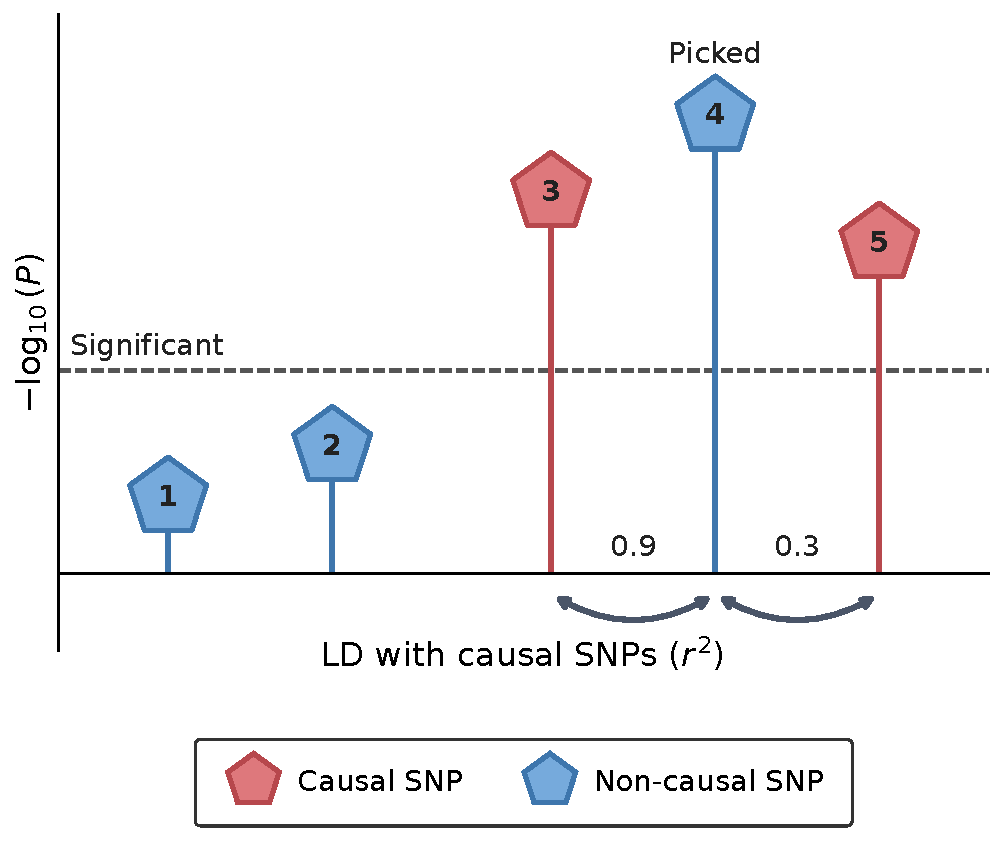
\includegraphics[width=\textwidth]{graphics/background_figures/ld_causal_plot.pdf}
        \label{fig:sub1}
    \end{subfigure}%
    \hfill
    \begin{subfigure}{0.45\textwidth}
        \caption{}
        \centering
        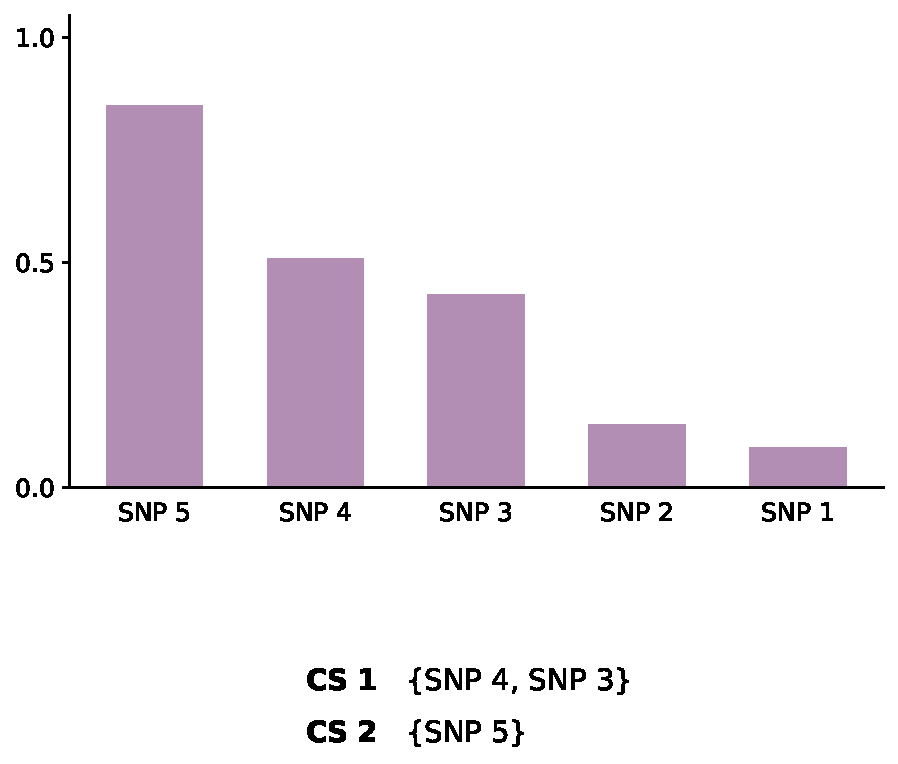
\includegraphics[width=\textwidth]{graphics/background_figures/fine_mapping_plot.pdf}
        \label{fig:sub2}
    \end{subfigure}
    
    \caption[Conceptual overview of the fine-mapping process highlighting the limitations of marginal association testing influenced by LD structure]{Conceptual overview of the fine-mapping process highlighting the limitations of marginal association testing influenced by LD structure. (a) Example of the correlation structure between causal and non-causal variants. The $y$-axis displays the significance of the marginal association testing. This example demonstrates that relying solely on a standard ranking of marginal associations fails to properly distinguish between causal and non-causal variants due to linkage disequilibrium. (b) The desired outcome of fine-mapping methods is the derivation of posterior inclusion probabilities for individual SNPs. These probabilities can then be used to construct credible sets (CS 1 and CS 2) with guaranteed false discovery control. This figure is adapted from \cite{FineMappingReview2025}.}
    \label{fig:fine_mapping_main_figure}
\end{figure}


\subsection{Statistical fine-mapping of genetic associations}

\label{sec:fine_mapping}

Building upon the preliminary screening provided by marginal association analyses, statistical fine-mapping aims to identify the causal genetic variants, typically within a local genomic window of length 1 Mb (one million base pairs). Overlapping windows are merged into a final set of loci ready for analysis \cite{FineMappingReview2025}. While the multiple regression framework serves as the foundation for these analyses, the primary challenge involves exploring the $2^P$ possible causal configurations within an associated locus containing $P$ genetic variants. To navigate this, fine-mapping methods are predominantly based on a Bayesian framework, which allows for incorporating prior assumptions about the genetic architecture of the trait, such as the expected number of causal variants per genomic window or the distribution of effect sizes that can further enhance the statistical power \cite{infinitesimalFineMapping2024}. Furthermore, such approaches can quantify probabilistic evidence in terms of \glspl{pip}, which can then be used to create disjoint credible sets. We define the \textit{$\alpha$-level credible set} as the minimal set of genetic variants that contains at least one causal variant with probability greater than or equal to $\alpha$. If we further define Bayesian FDR (bFDR) as the expected fraction of false discoveries under the posterior distribution of the model, then the following relationship holds between PIPs and bFDR (the proof of which can be found in Appendix \ref{Background_Appendix}):

\begin{lemma}[Bound on the Bayesian False Discovery Rate, adapted from \cite{Muller2004}]
Let $D$ be the observed GWAS data and $\mathcal{S}$ be a non-empty set of genetic variants selected as putative discoveries, with cardinality $|\mathcal{S}| > 0$. For every $j\in \mathcal{S}$, let $z_j \in \{0, 1\}$ be the unobserved, true causal indicator for variant $j$, and let $\text{PIP}_j = \mathbb{P}(z_j = 1 \mid D)$ be its PIP. Denoting the Bayesian False Discovery Rate of the set $\mathcal{S}$ as bFDR$(\mathcal{S})$, the following holds:

If there exists a constant $c \in [0, 1]$ such that $\text{PIP}_j \ge c$ for all variants $j \in \mathcal{S}$, then bFDR$(\mathcal{S}) \le 1 - c$.
\end{lemma}

Furthermore, it can be shown that to minimize posterior expected false negatives while strictly keeping the posterior expected false discovery proportion below a target threshold, the optimal decision rule is to rank and select all variants with a PIP above an appropriate threshold \cite{Muller2004}. Motivated by these results, we say a fine-mapping method is \textit{well-calibrated} if applying the thresholding rule $\text{PIP} \ge c$ guarantees that the observed \gls{fdr} is less than or equal to $1 - c$. In practice, the threshold $c = 0.95$ (yielding an observed $\text{FDR} \le 0.05$) is of primary interest.

Widely used frameworks for fine-mapping utilize different strategies to identify causal signals while maintaining computational efficiency:
\begin{itemize}
    \item Shotgun Stochastic Search with complexity reduction: Utilized by tools such as FINEMAP \cite{10.1093/bioinformatics/btw018}, this approach reduces the complexity of fitting a maximum likelihood estimator for a given configuration of hypothesized causal SNPs. Instead of scaling cubically with the total number of input SNPs, the complexity is reduced to cubic in the maximum number of hypothesized causal variants. This iterative procedure explores the search space by adding, deleting, or swapping a SNP within the current set at each step, enabling the identification of multiple causal signals per locus far more efficiently than exhaustive search methods.
    \item Sum of Single Effects (SuSiE) \cite{susie_original}: This framework reformulates the multiple regression model by expressing total genetic effects as a sum of a fixed number of single effects, where each component represents exactly one causal variant. The specific variable responsible for determining the location of each single effect is drawn from a multinomial distribution (typically uniform across all variants), while its non-zero coefficient is assumed to follow a normal distribution. The algorithm requires the user to input the maximum number of effects, while hyperparameters such as the residual Gaussian variance and prior effect variances are typically estimated directly from the data using an empirical Bayes approach that maximizes the variational evidence lower bound. This re-parameterization allows for Iterative Bayesian Stepwise Selection, a variational Bayes algorithm that avoids the need to search all possible SNP combinations. SuSiE offers linear computational complexity relative to the number of individuals and variants. More recent extensions of the SuSiE framework focus on using summary data \cite{susie} as the input to the algorithm and on fine-mapping multiple traits simultaneously \cite{SusieMultiTrait2026}.
\end{itemize}

One extension of the aforementioned approaches involves directly modeling background signals alongside SuSiE or FINEMAP via an infinitesimal model. Namely, standard fine-mapping frameworks usually assume strict sparsity, meaning that only a small number of variants causally contribute to the phenotype, and that all true causal signals are either included in, or highly tagged by, this sparse subset. However, failing to account for widespread and nonsparse genetic effects can lead to the miscalibration of posterior probabilities \cite{infinitesimalFineMapping2024}. To address this, methods such as SuSiE-Inf and FINEMAP-Inf \cite{infinitesimalFineMapping2024} explicitly incorporate an infinitesimal model alongside the sparse components, with a prior assuming that all variants contribute to the trait with equal variance. This combined architecture demonstrates superior calibration and tighter control over the replication failure rate, which serves as an approximate lower bound for the FDR. Additionally, one can further enhance the resolution of such analyses by integrating functional annotations, which provide prior information regarding the biological relevance of specific variants (e.g., coding changes or regulatory activity) \cite{FineMappingReview2025}. 

However, the scalability of these methods remains a critical bottleneck. Standard fine-mapping is typically performed locally, segmenting the genome into discrete, mostly independent LD blocks (e.g., 1--3 Mb regions) to make computation feasible. While this approach is sufficient for sparse genotyping arrays, the advent of whole-genome sequencing (WGS) within large-scale biobanks (e.g., UK Biobank, All of Us) presents a new challenge. In WGS settings, the density of variants increases dramatically, meaning that a single window may contain tens of thousands of variants. Moreover, this localized segmentation fundamentally fails to account for long-range LD. 

\newacronym{prs}{PRS}{Polygenic Risk Scores}
\newacronym{mcmc}{MCMC}{Markov chain Monte Carlo}
\section{Construction of polygenic risk scores}

\gls{prs} are quantitative measures that aggregate the effects of multiple genetic variants across the genome to estimate an individual's genetic predisposition to a particular trait or disease. The construction of PRS typically involves two main steps: (1) estimating the effect sizes of SNPs from GWAS summary statistics or individual-level data, and (2) aggregating these effects into a single score for each individual. The score for individual $i$ in the case of linear models is computed as
% The aggregation for individual $j$ in the case of linear models is computed as 
\begin{equation}
    \text{PRS}_i = \sum_{j=1}^{P} \hat{\beta}_j X_{i,j},
\end{equation}
where $\hat{\beta}_j$ is the estimated effect size of SNP $j$, $X_{i,j}$ is the known (column-normalized) genetic information of individual $i$ at SNP $j$, and $P$ is the total number of considered SNPs. Many of the commonly used methods for estimation of the effect sizes $\hat{\beta}_j$ are based on \gls{mcmc} sampling or variational Bayes inference. While MCMC offers asymptotically exact posterior distributions through stochastic sampling, it remains computationally demanding even when highly optimized; in contrast, variational Bayes approximates the posterior via deterministic optimization, trading a degree of theoretical exactness for gains in speed and scalability. Both frameworks yield PIPs that can also be used to construct credible sets of putative causal variants. In recent work \cite{Wu2024}, a genome-wide fine-mapping framework jointly leveraging functional genomic data was shown to outperform region-specific approaches, yielding more reliable causal variant identification and improved prediction across ancestry groups.

% In fact, recent work \cite{Wu2024} suggests that genome-wide fine-mapping approaches that integrate functional annotations can outperform earlier fine-mapping strategies, showing better calibration of posterior inclusion probabilities together with improved increased power and cross-ancestry predictive performance.

% In fact, recent work \cite{Wu2024} has shown that genome-wide fine-mapping with functional annotations improves over previously mentioned fine-mapping methods across multiple metrics including calibration of PIP values, mapping resolution, mapping precision, replication rate, and trans-ancestry phenotype prediction.

\subsection{Summary-level PRS methods}

\label{subsec:summary_level_prs}

\begin{figure}[htbp]
    \centering
    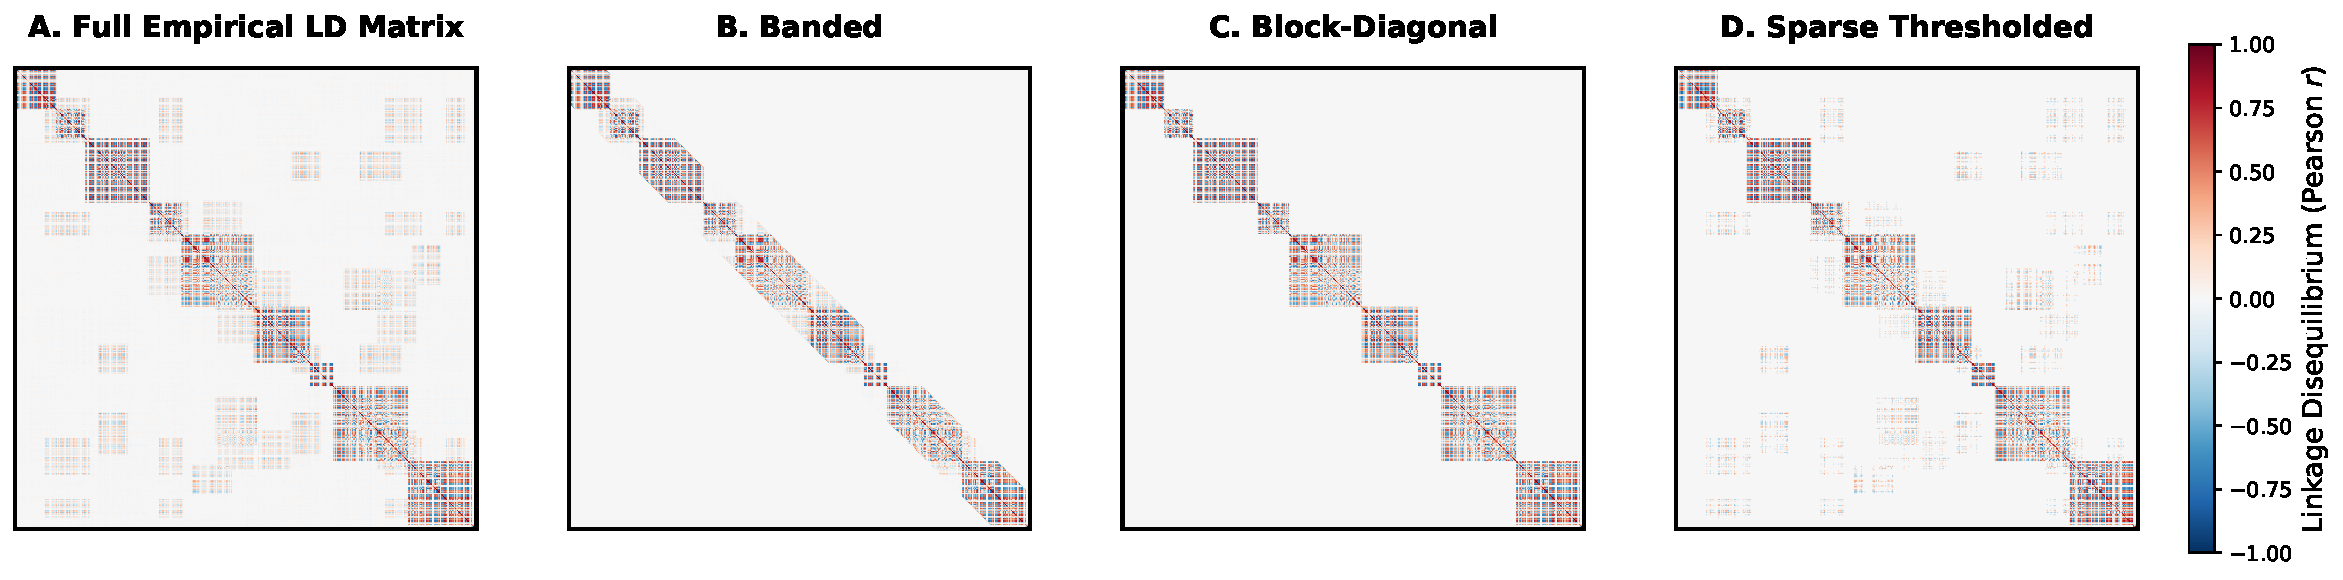
\includegraphics[width=\textwidth]{graphics/background_figures/ld_approximations_final.pdf}    
    \caption[Visual comparison of common LD matrix approximations]{\textbf{Visual comparison of common LD matrix approximations.} This figure illustrates the structure of an LD matrix within a single chromosome, as interchromosomal LD is conventionally assumed to be negligible. 
    \textbf{(A)} A full empirical LD matrix (Pearson correlation, $r$), showing dense local block structures alongside diffuse polygenic background correlations and complex longer-range LD signals. 
    \textbf{(B)} A banded approximation (e.g., utilized in LDpred models), where all correlations outside a strict bandwidth are set to zero. 
    \textbf{(C)} A block-diagonal approximation (e.g., utilized in SBayesR), where the genome is partitioned into independent LD blocks and all off-block correlations are set to zero. 
    \textbf{(D)} A sparse thresholded approximation, where all absolute correlations below a specified threshold are set to zero. While this approach preserves strong longer-range LD, it discards diffuse background correlations. Similar to the approximation errors introduced by matrix truncations, the zero inter-chromosomal LD assumption introduces further error.
    % Similar to the approximation errors introduced by these matrix truncations, assuming interchromosomal LD to be zero introduces further error. 
    This assumption is the main difference between models operating on full individual-level data and those relying on LD matrices and marginal effect sizes.}
    \label{fig:ld_approximations_final}
\end{figure}

Summary-statistic methods for constructing PRS utilize widely available GWAS summary statistics, which include marginal effect size estimates and their standard errors for each SNP, without requiring access to individual-level genotype data. They typically incorporate an external reference panel to account for the LD structure of the genome. Because the full genome-wide LD matrix is computationally intractable to store and invert, these methods rely on structural approximations---such as banded, block-diagonal, or sparse thresholded representations---to make inference feasible (Figure \ref{fig:ld_approximations_final}). Most modern implementations employ penalized regression techniques \cite{lassosum2017} or Bayesian frameworks to efficiently estimate effect sizes using either MCMC \cite{ldpred,sbayesr} or variational inference \cite{VIPRS2023,megaprs2021} approaches. In the remainder of this section, we give an overview of two widely used methods based on an MCMC approach: LDpred2 and SBayesR.

LDpred2 \cite{ldpred} is a Bayesian summary-level method that assumes a point-normal mixture prior for SNP effect sizes. Specifically, a learnable fraction of SNPs (treated as a hyperparameter) is assumed to be causal and assigned a Gaussian prior with equal variance across all causal variants, while the remaining non-causal variants have an effect size of exactly zero. LDpred2 employs a Gibbs sampler to estimate the posterior mean of the effect sizes. Its "auto" version bypasses the need for a validation dataset by estimating the fraction of causal SNPs and total heritability directly from the training data during the sampling iterations. The algorithmic time complexity scales linearly with the number of variants $P$, the number of Gibbs sampler iterations $N_{\text{it}}$, and the average number of variants within the window after an initial LD matrix pre-computation. Furthermore, the software utilizes a sparse matrix memory-mapping implementation in C++, which strictly bounds memory usage.

SBayesR \cite{sbayesr} is a summary-data-based multiple regression model that accommodates the varying degrees of polygenicity and effect size magnitudes inherent in complex traits. It generalizes the point-normal mixture prior of LDpred2 by utilizing a finite mixture of $L$ normal distributions combined with a point mass at zero, defined by the Dirac delta $\delta_0$, for the SNP effect sizes. The prior distribution for the effect $\beta_j$ of the $j$-th SNP is defined as:
\begin{equation}
\beta_j \sim (1-\lambda) \cdot \delta_0 + \lambda \cdot \sum_{l=1}^{L} \pi_l \cdot \mathcal{N}(\cdot, 0, \gamma_l \cdot \sigma_{\beta}^2),
\end{equation}
where $\lambda \in [0,1]$ is the sparsity rate, $(\pi_l)_{l=1}^L$ are the mixing probabilities of a causal SNP belonging to component $l=1,\dots,L$, $(\gamma_l)_{l=1}^L$ define the variance scaling factors.
%  and $\mathcal{N}(\cdot, \mu, \sigma^2)$ denotes the normal distribution with mean $\mu$ and variance $\sigma^2$. 
SBayesR operates with three non-spike components ($L=3$) whose variances form a geometric series with a factor of $10$. Posterior effects are estimated via a Gibbs sampler whose computational complexity scales linearly with the number of variants, the number of iterations, and the expected number of non-zero effects per iteration. This efficiency is achieved by exploiting a sparse representation of the LD structure and strictly updating only the non-zero effects during each iteration. 
% , the average number of non-zero elements per column in the LD matrix
\subsection{Individual-level PRS methods}

Individual-level inference methods for the construction of polygenic risk scores operate directly on genotype matrices rather than relying on aggregated summary statistics. By utilizing the complete genetic profile of each participant, these models can capture long-range correlation patterns between SNPs. However, this approach typically demands substantial computational resources and vast memory storage, especially as modern biobanks scale to hundreds of thousands of individuals. Additionally, strict data privacy regulations often restrict access to raw individual-level genotypes, making these methods less practical to the broader research community compared to methods that only require public summary statistics. 

Similar to the summary-level methods, most implementations employ penalized regression techniques \cite{snpnet2020,regenie} or Bayesian frameworks to efficiently estimate effect sizes using MCMC approaches \cite{BayesAB2010, BayesC2011, BayesRR2013, BayesR2015, Orliac2022}.

\subsection{Genetic architecture and predictive limits of complex traits}

The predictive accuracy of polygenic risk score methods is constrained by the genetic architecture of the target trait \cite{Chatterjee}. Here, genetic architecture refers to the underlying pattern of genetic contributions to a phenotype, including how many loci are involved, how large their effects are, and how those effects are distributed across the genome. Genetic architectures are often described as monogenic, oligogenic, or polygenic, depending on whether one, a few, or very many variants contribute to phenotypic variation \cite{genetic_architecture}. For traits with an oligogenic architecture, where a small set of variants has relatively large effects, standard regression or Bayesian approaches can readily identify the causal signals, allowing accurate prediction even from comparatively modest sample sizes. By contrast, for highly polygenic or omnigenic traits, genetic liability is spread over tens of thousands of variants, each with an almost negligible effect. In this setting, separating these tiny effects from sampling noise typically requires large, biobank-scale cohorts \cite{Chatterjee}. Moreover, because conventional PRS models are linear and additive, any variance arising from non-additive genetic components (such as dominance or epistasis) or from intricate gene-environment interactions is, by construction, outside their predictive scope. Traits such as standing height and body mass index are commonly used as exemplary traits in complex trait genetics, as they are among the most heritable, straightforward to measure, and strongly polygenic \cite{HTbig}.

Our understanding of the genomic regions underlying these traits has advanced considerably. Recent large-scale analyses, such as the association study of 5.4 million individuals of different ancestries by Yengo et al. \cite{HTbig}, have identified 12,111 independent SNPs significantly associated with height, collectively accounting for nearly all the common SNP-based heritability. These SNPs are concentrated in genomic segments spanning about 21\% of the genome. Providing a theoretical basis for such widespread genomic involvement, complementary research \cite{omnigenic} demonstrates that height is influenced by an extraordinarily large number of causal variants, each with a tiny effect size. Because these variants are spread so widely that almost every 100kb window contributes to the phenotypic variance, these findings strongly support the omnigenic model. Under this model, thousands of peripheral genes contribute to a phenotype by propagating regulatory effects through a few core biological pathways.

For highly polygenic traits such as height and BMI, most of the genetic signal lies not in protein-coding regions, but in non-coding regulatory elements that weakly modulate overall gene expression \cite{bmi_noncoding,yengo_meta-analysis_2018}. Driven by massive sample sizes, modern PRS methods have also made substantial progress in out-of-sample prediction accuracy for those traits. For standing height, state-of-the-art predictors report explaining up to 44.7\% \cite{HTbig} of the phenotypic variance in independent test cohorts of European ancestry. For BMI, where environmental and behavioral confounding is stronger, reported out-of-sample predictive accuracy plateaus at 17.6\% \cite{bmi_prs} of the phenotypic variance, as predicted using genetic data of around 5.1 million people. Unlike highly polygenic anthropometric traits, cardiometabolic traits like blood pressure and HbA1c yield significantly fewer independent associated loci, reflecting a sparser detectable genetic architecture where fewer regions achieve genome-wide significance (Table \ref{table:table2}).

For human height, 60\% to 80\% of the phenotypic variance in European ancestry is likely to be genetic \cite{missing_heritability_ht}, with a pedigree-based estimate of heritability reaching even 0.882 \cite{Wainschtein2026}. Whole-genome sequencing now estimates heritability at about 71\% using SNPs \cite{Wainschtein2026}. The genetic architecture of this captured variance is highly stratified: common variants drive 66\% of the pedigree-based heritability (compared to 14\% from rare variants), and non-coding regions contribute 80\% of the WGS-based heritability estimate (compared to 20\% from coding regions). The 20\% "missing" fraction of the total heritability is hypothesized to arise from ultra-rare (minor allele frequency $<0.001$) and structural variants not well tagged by SNPs, or non-additive genetic effects. 

To estimate the heritability parameter in whole-genome sequence data, researchers often rely on GREML-LDMS \cite{missing_heritability_ht}, which utilizes variance-component models to assess the aggregate contribution of different groups of variants. While successful in quantifying overall variance, this approach inherently requires stratifying variants based on allele frequency and linkage disequilibrium. In contrast, the gVAMP algorithm introduced in Chapter \ref{ch:gvamp} performs a joint analysis of rare and common variants within a unified, high-dimensional framework. By estimating the effect sizes of rare variants conditionally upon the common genetic background, gVAMP provides a methodology for both quantifying the variance attributable to rare variation at a much higher resolution and for effectively fine-mapping the underlying causal loci.

\section{Survival analysis}
Survival analysis provides a statistical framework for analyzing time-to-event or age-at-diagnoses data, characterized by the presence of censoring. While censoring can take several forms---such as left-censoring, where the event is known to have occurred prior to observation time, and right-censoring, where the study ends or the patient drops out before the event occurs---clinical data in the UK Biobank are predominantly right-censored. Hence, let the random variables $T$ and $C$ denote the true survival time and the censoring time, respectively. The observed data for individual $i$ consists of the pair $(t_i, \delta_i)$, where $t_i = \min(T_i, C_i)$ is the observed time and $\delta_i = \mathbb{I}(T_i \leq C_i)$ is the event indicator. The central object of interest is the hazard function $h(t)$, defined as the instantaneous rate of occurrence of the event at time $t$, conditional on the individual not having experienced the event until that time:

\begin{equation}
    h(t) = \lim_{\Delta t \to 0} \frac{P(t \le T < t + \Delta t \mid T \ge t)}{\Delta t}.
\end{equation}

\newacronym{coxph}{CoxPH}{Cox Proportional Hazards}
\subsection{Cox Proportional Hazards model}
The \gls{coxph} model \cite{coxPH1972} is a semi-parametric regression model that relates the hazard function for individual $i$ to a vector of covariates $\bm{x}_i \in \mathbb{R}^P$. The model assumes that the hazard for individual $i$ at time $t$ is the product of an unspecified baseline hazard $h_0(t)$ and an exponential multiplicative factor determined by the covariates:

\begin{equation}
    h(t \mid \bm{x}_i) = h_0(t) \exp(\bm{\beta}^\top \bm{x}_i),
\end{equation}

where $\bm{\beta} \in \mathbb{R}^P$ is a vector of regression coefficients, and $P$ is the number of covariates included in the study. Inference is typically performed by maximizing the partial likelihood $L(\bm{\beta})$, which eliminates the parameter $h_0(t)$. The partial likelihood is given by:

\begin{equation}
    L(\bm{\beta}) = \prod_{i: \delta_i = 1} \frac{\exp(\bm{\beta}^\top \bm{x}_i)}{\sum_{j \in \mathcal{R}(t_i)} \exp(\bm{\beta}^\top \bm{x}_j)},
\end{equation}

where $\mathcal{R}(t_i) = \{j : t_j \ge t_i\}$ represents the risk set (the set of individuals still at risk of experiencing the event) at time $t_i$. In practice, the log-partial likelihood, $\ell(\bm{\beta}) = \log L(\bm{\beta})$, is maximized due to its numerical properties. Importantly, the negative log-partial likelihood, $-\ell(\bm{\beta})$, is strictly convex with respect to $\bm{\beta}$, provided the covariate matrix is of full rank. While there is no closed-form analytical solution for the estimator $\hat{\bm{\beta}}$, this strict convexity guarantees a unique global minimum for the negative log-partial likelihood. Consequently, numerical optimization algorithms, such as the Newton-Raphson method, can reliably converge to the unique estimate of $\hat{\bm{\beta}}$.

While the partial likelihood eliminates the baseline hazard $h_0(t)$ to estimate $\bm{\beta}$, this nuisance parameter can be recovered using the Breslow estimator \cite{Breslow1974CovarianceAO}. For a given set of coefficients, the Breslow estimator provides a non-parametric estimate of the cumulative baseline hazard function $H_0(t) = \int_0^t h_0(u) \ du$. It is defined as a step function that increases at each observed age-at-onset time $t_i$:
\begin{equation}
    \hat{H}_0(t) = \sum_{t_i \le t} \frac{\delta_i}{\sum_{j \in \mathcal{R}(t_i)} \exp(\bm{\beta}^\top \bm{x}_j)}.
\end{equation}
This estimator of $H_0$, and by extension of $h_0$, is particularly useful for predicting absolute survival probabilities for new individuals. 
% By combining the estimated coefficients $\hat{\bm{\beta}}$ with the Breslow estimator, the survival function for a subject with covariates $\bm{x}$ is expressed as $\hat{S}(t \mid \bm{x}) = \exp(-\hat{H}_0(t) \exp(\hat{\bm{\beta}}^\top \bm{x}))$.

\subsection{Regularization: Cox-Lasso and Stability Selection}
In high-dimensional settings where the number of variables $P$ exceeds the sample size, or where variables are highly correlated, standard maximum likelihood estimation of the Cox model becomes ill-posed and prone to overfitting. To address this, the Cox-Lasso integrates the $\ell_1$ penalty into the optimization objective \cite{tibshirani_lasso_1997,Simon2011}. The coefficients are estimated by minimizing the negative log-partial likelihood with a penalty term:

\begin{equation}
    \hat{\bm{\beta}}_{\text{cox-lasso}} = \operatorname*{arg\,min}_{\bm{\beta}} \left[ - \log L(\bm{\beta}) + \lambda_{\text{reg}} \sum_{j=1}^P |\beta_j| \right].
\end{equation}

Here, $\lambda_{\text{reg}} \ge 0$ is a hyperparameter that controls the strength of regularization. The $\ell_1$ penalty encourages sparsity, forcing the coefficients of non-informative variables to be exactly zero, thereby performing simultaneous variable selection and parameter estimation. While Cox-Lasso provides sparse solutions, the specific set of selected variables can be unstable in the presence of noise or high collinearity. 

While Cox-Lasso provides sparse solutions, it has a known limitation in the presence of high collinearity: it tends to arbitrarily select only one variable from a group of highly correlated features, making the chosen set unstable. One approach to address this issue is to utilize the Cox Elastic Net \cite{Simon2011}, which linearly combines the $\ell_1$ and $\ell_2$ (ridge) penalties. The addition of the $\ell_2$ penalty introduces a "grouping effect", encouraging highly correlated variables to be selected or shrunk together. The Elastic Net objective is given by:

\begin{equation}
    \hat{\bm{\beta}}_{\text{cox-en}} = \operatorname*{arg\,min}_{\bm{\beta}} \left[ - \log L(\bm{\beta}) + \lambda_{\text{reg}} \left( \alpha \sum_{j=1}^P |\beta_j| + \frac{1-\alpha}{2} \sum_{j=1}^P \beta_j^2 \right) \right],
\end{equation}

where $\alpha \in [0, 1]$ controls the balance between the Lasso ($\alpha=1$) and Ridge ($\alpha=0$) penalties. Such approach has been successfully applied to relating blood plasma protein levels to disease onset times in the UK Biobank \cite{Smith2025}.

Alternatively, to improve the robustness of feature selection in Cox-Lasso, Stability Selection \cite{meinshausen_stability_2010} can be employed. This method involves running the Cox-Lasso algorithm on $B$ random subsamples of the data (typically $B \ge 100$). For a given regularization level $\lambda_{\text{reg}}$, the selection probability $\hat{\Pi}_j^{\lambda_{\text{reg}}}$ for variable $j$ is calculated as the frequency with which the variable is selected across the subsamples:

\begin{equation}
    \hat{\Pi}_j^{\lambda_{\text{reg}}} = \frac{1}{B} \sum_{k=1}^B \mathbb{I}(\hat{\beta}_{j}^{(k)} \neq 0),
\end{equation}

where $\hat{\beta}_{j}^{(k)}$ is the coefficient estimate from the $k$-th subsample. Variables are deemed stable and are retained only if their selection probability exceeds a predefined threshold $\pi_{\text{thr}}$ for at least one choice of $\lambda_{\text{reg}}$. This approach reduces the influence of spurious correlations arising from sampling noise and provides control over the finite-sample family-wise error rate.

% This approach effectively filters out false positives resulting from stochastic noise and provides control over the finite-sample family-wise error rate.

\newacronym{aft}{AFT}{Accelerated Failure Time}
\subsection{Parametric models}
When the proportional hazards assumption of the Cox model is not satisfied or when there is interest in directly modeling the survival time distribution, Accelerated Failure Time models offer a robust alternative. Parametric approaches explicitly parameterize the baseline hazard, making them highly effective for capturing distinct biological risk profiles and increasing statistical power. For example, Weibull regression \cite{Weibull1951ASD} captures monotonic risk changes and has been successfully applied to modeling human age-at-onset traits \cite{Ojavee2021-zu}. Similarly, the Gompertz model is used for mapping polygenic influences on aging and lifespan \cite{Timmers2020}, while log-normal and log-logistic models are utilized for complex genetic traits characterized by a peak-and-decline onset pattern, such as specific neurogenetic disorders \cite{Tezenas2014}.

\subsection{Deep learning approaches to survival analysis}

In recent years, advancements in neural network architectures and the increasing scale of omics datasets have driven the development of deep learning approaches to survival analysis. DeepSurv \cite{katzman_deepsurv_2018}, for instance, extends the semi-parametric Cox proportional hazards model. To overcome the expressivity limitations of linear models, it replaces the standard linear predictor $\bm{\beta}^\top \bm{x}_i$ with a nonlinear function $f_{\bm{\theta}}(\bm{x}_i)$, parameterized by a neural network with weights $\bm{\theta}$. The hazard function in DeepSurv is defined as:
\begin{equation}
h(t|\bm{x}_i) = h_0(t) \exp(f_{\bm{\theta}}(\bm{x}_i)).
\end{equation}
% By minimizing the negative log partial likelihood to optimize its weights, the network effectively learns complex and nonlinear representations of high-dimensional covariates while preserving the hazard ratio framework of the original Cox model. 
Because the nonlinear formulation of $f_{\bm{\theta}}(\cdot)$ renders the negative log-partial likelihood non-convex with respect to the network weights $\bm{\theta}$, exact global minimization is mathematically intractable. Instead, DeepSurv relies on approximate minimization via stochastic gradient-based optimization algorithms. Through this optimization, the network extracts complex nonlinear features while preserving the original Cox hazard ratio interpretation. In terms of applications to biological data, researchers have been successful in integrating multi-omics data and clinical covariates to predict patient survival trajectories. For example, DeepSurv has been applied to integrate multi-genomic profiles for predicting survival time across several cancer types \cite{deepsurv_application2022,Chaudhary2018}. Cox-nnet \cite{coxnnet2018} was developed for the analysis of RNA sequencing data and has successfully identified critical biological drivers, including the predictive significance of specific metabolic pathways in cancer.
% For example, DeepSurv has been applied to integrate multi-genomic profiles for predicting survival time in head and neck squamous cell carcinoma \cite{deepsurv_application2022} and other complex cancers \cite{Chaudhary2018}. 
% Cox-nnet \cite{coxnnet2018} has been designed to evaluate RNA sequencing data and has identified critical biological drivers, such as the prognostic role of the pentose phosphate pathway in kidney cancer. 
Building on the need for biological interpretability, specialized architectures like Cox-PASNet \cite{coxpasnet2018} have utilized pathway-based sparse deep neural networks to evaluate the prognostic impact of specific genetic pathways on patient mortality. However, many contemporary deep learning frameworks for survival analysis, such as CoxTime \cite{CoxTime2019}, CoxCC \cite{CoxTime2019}, SurvTRACE \cite{SurvTrace2022} and PCHazard \cite{PChazard2021}, have largely been validated on smaller clinical datasets where the sample-to-feature ratio is relatively high.

\newacronym{iid}{i.i.d.}{independent and identically distributed}
\newacronym{amp}{AMP}{Approximate Message Passing}
\newacronym{vamp}{VAMP}{Vector Approximate Message Passing}
\newacronym{em}{EM}{Expectation-Maximization}
\section{Overview of approximate message passing}

The \gls{amp} framework \cite{DMM09,rangan_vector_2019,feng2022unifying} provides a powerful class of iterative algorithms for Bayesian inference, which possesses several attractive theoretical properties (as summarized in \cite{Depope2026}). First, the framework is flexible, accommodating a vast array of prior distributions. Second, the empirical distribution of the iterates within this framework, in the high-dimensional limit, can be exactly tracked using a simple recursion known as \textit{state evolution} \cite{Bayati2011}. Third, this state evolution machinery facilitates the precise derivation of joint association test statistics \cite{montanari2017estimation,feng2022unifying}. Finally, under appropriate conditions, AMP provably achieves Bayes-optimal inference \cite{barbier-mmse-glm-pnas,montanari2017estimation,barbier2023fundamental,zhang2026optimal}.

AMP was originally proposed for the linear compressed sensing problem \cite{DMM09, Bayati2011, krzakala2012}, assuming an \gls{iid} Gaussian design matrix. Empirical evidence \cite{donoho2009observed, monajemi2013deterministic} suggests that phase transition results and state evolution apply to a broader range of design matrices. This includes highly structured transforms paired with a Gaussian signal prior \cite{dudeja2022universality} as well as matrices characterized by heavy-tailed distributions and heterogeneous variances \cite{Wang22AMPUniversality}.

In the continuation of this subsection, we first provide an informal overview of the AMP framework applied to the Bayesian linear regression problem inspired by \cite{feng2022unifying}.  

We begin with the well-known LASSO optimization problem under the assumption that the noise variance is known and equal to $1$. For a given regularization parameter $\lambda > 0$, the estimator of the effect sizes $\hat{\bm{\beta}}$ is defined as  
\begin{align}
    \label{Lasso_problem}
    \hat{\bm{\beta}} \in \text{argmin}_{\bm{\beta} \in \mathbb{R}^P} \bigg\{ \frac{1}{2} \lVert \bm{y} - \bm{X} \bm{\beta} \rVert^2 + \lambda \lVert \bm{\beta} \rVert_1 \bigg\}.
\end{align}
This formulation admits a Bayesian interpretation: it can be seen as a posterior mode estimation problem for a linear regression model with independent $\text{Laplace}(0,1/\lambda)$ priors on the coefficients.  

A classical algorithm for solving \eqref{Lasso_problem} is the iterative soft-thresholding algorithm (ISTA) \cite{ISTA}, which initializes the estimate $\hat{\bm{\beta}}_0 = \mathbf{0}$ and then performs the following iterations:
\begin{equation}
\begin{split}
    \hat{\bm{r}}_t &= \bm{y} - \bm{X} \hat{\bm{\beta}}_t, \\
    \hat{\bm{\beta}}_{t+1} &= \text{ST}_{\lambda \eta_k} \!\left( \hat{\bm{\beta}}_t + \eta_t \bm{X}^\top \hat{\bm{r}}_t \right), 
    \quad t \in \mathbb{N}_0,
\end{split}
\end{equation}
where $\hat{\bm{r}}_t$ is the residual at iteration $t$, $\eta_t > 0$ is a deterministic step size, and $\text{ST}_\tau : \mathbb{R} \to \mathbb{R}$ denotes the \emph{soft-thresholding operator} defined by  
\begin{equation}
\text{ST}_\tau(w) = \operatorname{sgn}(w) \, (|w| - \tau)_+, 
\quad (a)_+ = \max\{a, 0\}.
\end{equation}

An accelerated variant of ISTA, dubbed the \emph{fast iterative shrinkage-thresholding algorithm} (FISTA) \cite{FISTA}, shares structural similarities with the AMP methods we present next. However, rather than using momentum like FISTA, AMP modifies the ISTA framework by introducing a memory correction term, commonly referred to as the \emph{Onsager correction term}. Its iterations take the following form:

\begin{equation}
\label{FISTA}
\begin{aligned}
    \hat{\bm{r}}_t &= \bm{y} - \bm{X} \hat{\bm{\beta}}_t + \frac{\lVert \hat{\bm{\beta}}_t \rVert_0}{n} \, \hat{\bm{r}}_{t-1}, \\
    \hat{\bm{\beta}}_{t+1} &= \text{ST}_{\tau_{t+1}} \!\left( \hat{\bm{\beta}}_t + X^\top \hat{\bm{r}}_t \right), 
    \quad t \in \mathbb{N},
\end{aligned}
\end{equation}
where $\tau_{t+1} > 0$ is a deterministic threshold at iteration $(t+1)$, the corresponding soft-thresholding operator is applied component-wise and $\lVert \hat{\bm{\beta}}_t \rVert_0$ denotes the number of non-zero entries in $\hat{\bm{\beta}}_t$.  
In contrast to ISTA, the residual $\hat{\bm{r}}_t$ here includes a memory correction term, which is crucial for enabling an exact characterization of the empirical distribution of the iterates; if one chooses the threshold sequence $(\tau_t)_t$ appropriately \cite{feng2022unifying}, then this AMP algorithm converges to the solution of the LASSO problem in \eqref{Lasso_problem}.  

Returning to the previously mentioned LASSO formulation, one may wish to replace the Laplace prior with a more flexible alternative, such as a spike-and-slab prior, where the slab component is a Gaussian mixture. In the AMP framework, this modification can be achieved by replacing the soft-thresholding operator in \eqref{FISTA} with the conditional expectation under the spike-and-slab prior, and adjusting the residual correction term accordingly as the conditional variance. This yields an AMP-based framework for Bayesian regression under spike-and-slab priors, where the prior parameters can be updated iteratively via the \gls{em} algorithm \cite{EMGAMP2012}. 
% However, when applied to real-world design matrices characterized by non-zero means, column correlations, or, more generally, ill-conditioned singular value spectra---such as those frequently encountered in genomic studies---standard AMP often suffers from severe instabilities and diverges \cite{vila_adaptive_2015,AMP_convergence}. To mitigate these convergence issues, several algorithmic modifications were initially proposed in the literature. These approaches include introducing damping mechanisms to smooth the iterative updates and prevent oscillations \cite{vila_adaptive_2015}, applying mean-removal operations \cite{vila_adaptive_2015}, and utilizing sequential updating schemes such as SwAMP \cite{SweptAMP2015}. While these stabilization techniques improved empirical convergence for moderately ill-conditioned matrices, they often lacked precise theoretical performance characterizations via state evolution and remained insufficient for highly correlated and structured data. To accommodate a wider class of design matrices, \gls{vamp} was introduced in \cite{rangan_vector_2019}. Its theoretical guarantees hold for any right-orthogonally invariant design matrix, where the right singular vectors are uniformly distributed in the group of orthogonal matrices.

However, when applied to real-world design matrices characterized by non-zero means, column correlations, or, more generally, ill-conditioned singular value spectra---such as those frequently encountered in genomic studies---standard AMP often suffers from severe instabilities and diverges \cite{vila_adaptive_2015,AMP_convergence}. To mitigate these convergence issues, several algorithmic modifications were initially proposed in the literature. These approaches include introducing damping mechanisms to smooth the iterative updates and prevent oscillations \cite{vila_adaptive_2015}, applying mean-removal operations \cite{vila_adaptive_2015}, and utilizing sequential updating schemes such as SwAMP \cite{SweptAMP2015}. While these stabilization techniques improved empirical convergence for moderately ill-conditioned matrices, they often lacked precise theoretical performance characterizations via state evolution and remained insufficient for highly correlated and structured data. To accommodate a wider class of design matrices, \gls{vamp} was introduced in \cite{rangan_vector_2019}. Its theoretical guarantees hold for any right-orthogonally invariant design matrix in the large-system limit, where the right singular vectors are uniformly distributed in the group of orthogonal matrices. Furthermore, despite these asymptotic guarantees, we note that in many practical, finite-dimensional applications, \gls{vamp} itself needs to be damped, employing schemes such as those discussed in \cite{VAMP_MRI}.

At their core, both algorithm families iteratively construct estimates of the signal that can be decoupled into the true signal plus independent Gaussian noise. More precisely, at iteration $t$, in the high-dimensional limit, this effective observation takes the form:
\begin{equation}
    \bm{r}_t = \mu_t \bm{\beta} + \bm{w}_t,
\end{equation}
where $\mu_t$ is a deterministic scalar gain (simplifying to $\mu_t = 1$ for VAMP and standard AMP for linear models) and $\bm{w}_t \sim \mathcal{N}(\mathbf{0}, \gamma_{t}^{-1} \bm{I})$ represents independent Gaussian noise. The algorithms keep the noise $\bm{w}_t$ independent of $\bm{\beta}$ through the \emph{Onsager correction}, a memory term that subtracts a scaled version of the previous iteration's measurement. Without this correction, the noise would become correlated with the design matrix and the signal, violating the Gaussian assumption. Because this independent error structure is preserved, state evolution maps the high-dimensional dynamics of the algorithm onto a simple, deterministic sequence. This allows us to track macroscopic observables—such as the mean squared error—and characterize the algorithm's asymptotic performance iteration-by-iteration without executing the high-dimensional matrix updates. Furthermore, because state evolution precisely quantifies the noise precision $\gamma_t$ at each iteration, one can design optimal denoisers tailored to a specific inference problem. By applying the conditional expectation (the posterior mean estimator) matched to this exact Gaussian noise level, the framework yields Bayes-optimal (V)AMP algorithms.

\subsection{Expectation-Maximization Vector Approximate Message Passing}

Algorithm \ref{EMVAMP} outlines the Expectation-Maximization Vector Approximate Message Passing (EM-VAMP). The framework partitions the complex global estimation of the effect sizes into two computationally tractable modules. The first module, dubbed the \textit{denoising step}, utilizes prior distributional assumptions on the effect sizes. The second module, designated as the \textit{Linear Minimum Mean Squared Error (LMMSE) estimation step}, ensures consistency with the data by directly incorporating the design matrix and the observed outcomes.

To clarify the mechanics of EM-VAMP at iteration $t>0$, we interpret the parameters of the denoising module (the LMMSE module is analogous). The previous LMMSE step at iteration $(t-1)$ provides the denoising module with a noisy input $\bm{r}_{1,t}$. This vector acts as a measurement of the true signal $\bm{\beta}$ corrupted by Gaussian noise, behaving asymptotically as $\bm{r}_{1,t} \sim \mathcal{N}(\bm{\beta}, \gamma_{1,t}^{-1} \bm{I})$. Here, the scalar $\gamma_{1,t}$ represents the asymptotic precision (or inverse variance) of this measurement. The denoising module uses $\bm{r}_{1,t}$ to compute $\hat{\bm{\beta}}_{1,t}$ utilizing prior information on $\bm{\beta}$. This estimates the posterior mean when the denoising function is the conditional expectation. The scalar $\alpha_{1,t}$ measures the empirical divergence of this estimator to construct the Onsager correction. This term decouples errors, ensuring that they remain strictly Gaussian and independent of the true signal by subtracting correlated information from the previous step. Finally, the EM algorithm dynamically updates $\Theta_t$, representing the prior distribution hyperparameters, by utilizing the independence and Gaussianity of the errors to construct a likelihood function.

To enhance the numerical stability of EM-VAMP, the iterates can be damped—replaced by a convex combination of current and previous values. This approach can be applied directly to signal estimates $\hat{\bm{\beta}}_{1,t}$ and precisions $\gamma_{1,t}$~\cite{rangan_vector_2019}, or to the auxiliary vectors $\bm{r}_{1,t}$ and $\bm{r}_{2,t}$ and their associated noise precisions $\gamma_{1,t}$ and $\gamma_{2,t}$~\cite{VAMP_MRI,sarkar2021mri}. Further robustness is achieved through variance auto-tuning, which jointly re-estimates the precision $\gamma_{1,t}$ alongside EM updates of the prior distribution parameters~\cite{RigorousDynamics2017}. When an explicit singular-value decomposition (SVD) of the sensing matrix is computationally prohibitive, the Onsager correction can be approximated using Hutchinson's trace estimator~\cite{schniter2021gampmatlab}. Similarly, the LMMSE step can be executed via a warm-started conjugate-gradient solver~\cite{schniter2021gampmatlab, skuratovs2022warmstarting}, effectively bypassing the need for an SVD. These techniques, alongside a diverse array of prior models—including spike-and-slab, (complex-valued) Gaussian mixtures, and Laplacian priors—are implemented in the open-source \texttt{GAMPmatlab} toolbox~\cite{schniter2021gampmatlab} developed in the MATLAB programming language.

EM-VAMP algorithm can be formulated via a constrained variational inference approach \cite{LearningFreeEnergies2018}. Instead of computing the intractable exact posterior with a single distribution, this Expectation Consistent (EC) framework introduces three separate tractable densities. The density $b_1$ relates to the prior, $b_2$ relates to the likelihood, and $q$ acts as a shared reference density. Rather than forcing these three distributions to be perfectly identical, the framework optimizes the energy function, defined for hyperparameters $\bm{\theta} = (\theta_1, \theta_2)$ as:
\begin{equation}
    J(b_1, b_2, q, \bm{\theta}) = D_1(b_1, \theta_1) + D_2(b_2, \theta_2) + H(q),
\end{equation}
where $H(q)$ represents the differential entropy of the reference density $q$. The terms $D_1(b_1, \theta_1)$ and $D_2(b_2, \theta_2)$ are Kullback-Leibler (KL) divergences where the first divergence, $D_1$, measures the distance between the belief $b_1$ and the signal prior distribution parameterized by $\theta_1$, which forces the density to align with the assumed prior structure of the coefficients. The second divergence, $D_2$, measures the distance between the distribution $b_2$ and the observational likelihood parameterized by $\theta_2$, ensuring the density closely matches the observed data. Furthermore, the framework imposes relaxed moment-matching constraints instead of requiring the densities to match exactly. Namely, by adapting the notation $\bm{\beta}$ for the unknown vector of coefficients, these constraints can be formulated as follows:
\begin{equation}
\begin{gathered}
\mathbb{E}[\bm{\beta} \mid b_1] = \mathbb{E}[\bm{\beta} \mid b_2] = \mathbb{E}[\bm{\beta} \mid q], \\ 
\mathbb{E}[\lVert \bm{\beta} \rVert^2 \mid b_1] = \mathbb{E}[\lVert \bm{\beta} \rVert^2 \mid b_2] = \mathbb{E}[\lVert \bm{\beta} \rVert^2 \mid q].
\end{gathered}
\end{equation}
The fixed points of the EM-VAMP algorithm correspond precisely to the stationary points of this constrained energy minimization. A more general form of EM-VAMP, designed for generalized linear models (GLMs) and capable of utilizing general denoising functions, is presented in Algorithm \ref{EMVAMP-GLM}. In a GLM, the observations $\bm{y}$ depend on the coefficients $\bm{\beta}$ through a non-linear likelihood applied to the linear predictor $\bm{z} = \bm{X} \bm{\beta}$. Consequently, the main architectural difference from standard VAMP is the introduction of an additional set of denoising and LMMSE steps to perform explicit inference on the transformed variables $\bm{z}$ alongside the coefficients $\bm{\beta}$.

\begin{breakablealgorithm}{Expectation-Maximization Vector Approximate Message Passing}{Expectation-Maximization Vector Approximate Message Passing \cite{LearningFreeEnergies2018}}{EMVAMP}
    \begin{algorithmic}[1]
        \STATE \parbox[t]{\dimexpr\linewidth-2\algorithmicindent}{% 
        {\bfseries Input:} design matrix $\bX \in \mathbb{R}^{N \times P}$, number of VAMP iterations $N_{\text{it}}$, initial estimate of effect sizes $\bm{r}_{1,0} \in \mathbb{R}^P$, initial estimate of effect sizes precision $\gamma_{1,0} \ge 0$, initial estimate of noise precision $\gamma_{\epsilon, 0} \ge 0$, initial set of parameters defining the prior distribution $\Theta_{0}$}
        \FOR{$t = 0, 1,\dots, N_{\text{it}}$}
            \STATE {\bfseries Denoising step}
            \STATE \text{EM} update of the prior distribution parameters $\Theta$, called $\Theta_t$

            \STATE $\hat{\bm{\beta}}_{1,t} = \mathbb{E}[\bm{\beta} | \bm{r}_{1,t} = \bm{\beta} + \mathcal{N}(0, \gamma_{1,t}^{-1}\bm{I}), \gamma_{1,t}, \Theta_{t}]$
            \STATE $\alpha_{1,t} = \gamma_{1,t} \cdot \langle \text{Var}[\bm{\beta}|\bm{r}_{1,t} = \bm{\beta} + \mathcal{N}(0, \gamma_{1,t}^{-1}\bm{I}), \gamma_{1,t}, \Theta_{t}] \rangle$
            \STATE $\gamma_{2,t} = \gamma_{1,t} \cdot (1 - \alpha_{1,t}) / \alpha_{1,t}$ 
            \STATE $\bm{r}_{2,t} = (\hat{\bm{\beta}}_{1,t} - \alpha_{1,t} \bm{r}_{1,t}) / (1-\alpha_{1,t})$
            \item[]
            \STATE \textbf{LMMSE step}
            \STATE { \text{EM update of the estimate of } $\gamma_{\epsilon}$\text{, called } $\gamma_{\epsilon,t}$ }
            \STATE $\hat{\bm{\beta}}_{2,t} =  ( \gamma_{\epsilon,t} \bm{X}^\top\bm{X} + \gamma_{2,t} \bm{I} )^{-1} ( \gamma_{\epsilon,t} \bm{X}^\top \bm{y} + \gamma_{2,t} \bm{r}_{2,t} )$ 
            \STATE $\alpha_{2,t} = \gamma_{2,t} \cdot \text{Tr}[(\gamma_{\epsilon,t} \bm{X}^\top\bm{X} + \gamma_{2,t}\bm{I})^{-1}] / P$
            \STATE $\gamma_{1,t+1} = \gamma_{2,t} \cdot (1-\alpha_{2,t}) / \alpha_{2,t}$
            \STATE $\bm{r}_{1,t+1} = (\hat{\bm{\beta}}_{2,t} - \alpha_{2,t} \bm{r}_{2,t}) / (1-\alpha_{2,t})$ 
        \ENDFOR
        \STATE \textbf{return} $\hat{\bm{\beta}}_{1,t}$
    \end{algorithmic}
\end{breakablealgorithm}

% \newpage

\section{What is this thesis about?}
This thesis addresses the following two challenges in computational omics:
\begin{enumerate}
	\item Can we scale joint effect inference to tens of millions of variants to enable high-resolution fine-mapping and accurate polygenic risk prediction at the full-biobank scale? 
	\item Can we design a parametric survival model framework for proteomics data by incorporating censoring information to improve biomarker selection accuracy over the current state-of-the-art methods?
\end{enumerate}

This thesis provides affirmative answers to both questions. Chapter \ref{ch:gvamp} introduces \textit{gVAMP} (genomic Vector Approximate Message Passing), a computational framework that addresses the first challenge of scalability, while also exhibiting state-of-the-art predictive performance. Chapter \ref{ch:vampw} presents \textit{vampW} (VAMP for Weibull models), a novel method for state-of-the-art variable selection that addresses the second question by enabling parametric survival analysis for proteomics. Finally, Chapter \ref{ch:limitations_perspectives} discusses the limitations and future perspectives of the (Vector) Approximate Message Passing framework in computational omics. It introduces a summary-statistics version of gVAMP and outlines a potential transfer learning framework for cross-ancestry polygenic risk score prediction.
